\section{Experiments} \label{subsec:experiments}
In this section, we first discuss our novel dataset, followed by experiments on the outputs learned by our model. In particular, we evaluate the trustworthy comment embeddings on the comment ranking task while we qualitatively evaluate user reliabilities and word embeddings. For brevity, we focus the qualitative analysis on our largest subreddit, askscience.
\subsection{Dataset} \label{subsec:dataset}
We evaluate our model on a widely popular discussion forum Reddit. Reddit covers diverse topics of discussion and is challenging due to the prevalence of noisy responses.

\begin{table}[tbh]
  \centering
\begin{tabular}{  p{20mm}| r | r | r | r | r | r}
\toprule
  Dataset & Created & $N$ & \textbf{$N_e$} & \textbf{$M$} & \textbf{$\vert a_{m,e} \vert$} & \textbf{$\vert w_{m,n} \vert $} \\ %\hline
  \midrule
 *Docs & 07/13 & 3,334 & 286 & 17,342 & 10,389 & 53.5 \\
 *Science & 04/10 & 73,463 & 2,195 & 100,237 & 70,108 & 74.0\\
*Historians & 08/11 & 27,264 & 296 & 45,650 & 30,268 & 103.4 \\
 \bottomrule
\end{tabular}
\caption{\label{tab:redditdata} Dataset statistics for the subreddit communities. The symbol meaning are as follows: $N$ and $M$ denotes total users and posts respectively; $N_e$: number of experts; $\vert a_{m, e} \vert$: number of posts with at least one expert comment; $\vert w_{m, n} \vert$: average comment word length. }
\end{table}

We specifically tested on \emph{Ask*} subreddits as they are primarily used to seek answers to a variety of topics from mundane issues to serious medical concerns. In particular, we crawled data from three subreddits, /r/askscience, /r/AskHistorians, and /r/AskDocs from their inception until October 2017 \footnote{\url{praw.readthedocs.io/en/latest/} }. While these subreddits share the same platform, the communities differ vastly, see Table \ref{tab:redditdata}. We preprocessed the data by removing uninformative comments and posts with either less than ten characters or containing only URLs or with a missing title or author information.
We removed users who have posted less than two comments and also submissions with three or fewer comments. To handle sparsity, we treated all users with a single comment as "UNK".


\begin{figure}[tbh]
\centering
  \begin{subfigure}{0.5\textwidth}
  \centering
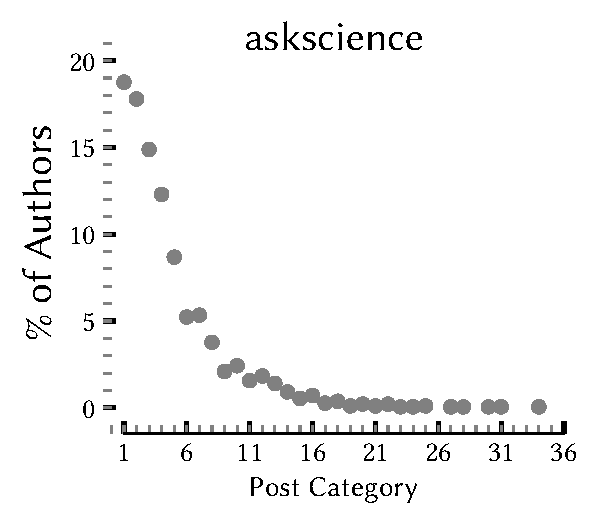
\includegraphics[scale=0.62]{images/Flair_frequency.pdf}
\end{subfigure}%
  \begin{subfigure}{0.5\textwidth}
  \centering
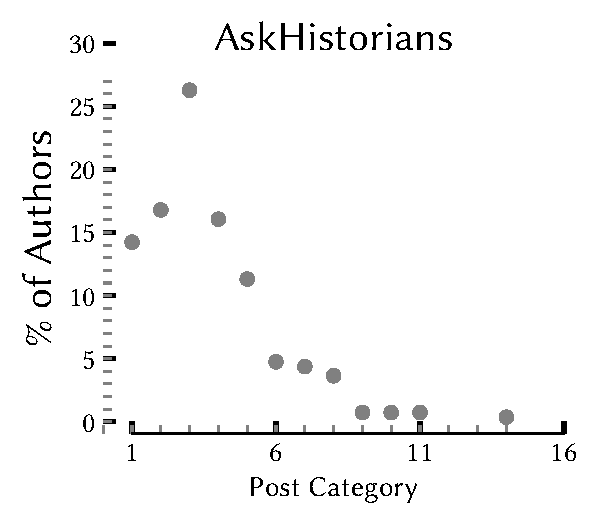
\includegraphics[scale=0.62]{images/Flair_frequency_askhistory.pdf}
\end{subfigure}
\caption{Frequency plot of \% of authors commenting on the post with unique submission flairs.}
\label{fig:flair}
\end{figure}

\begin{figure}
  \centering
  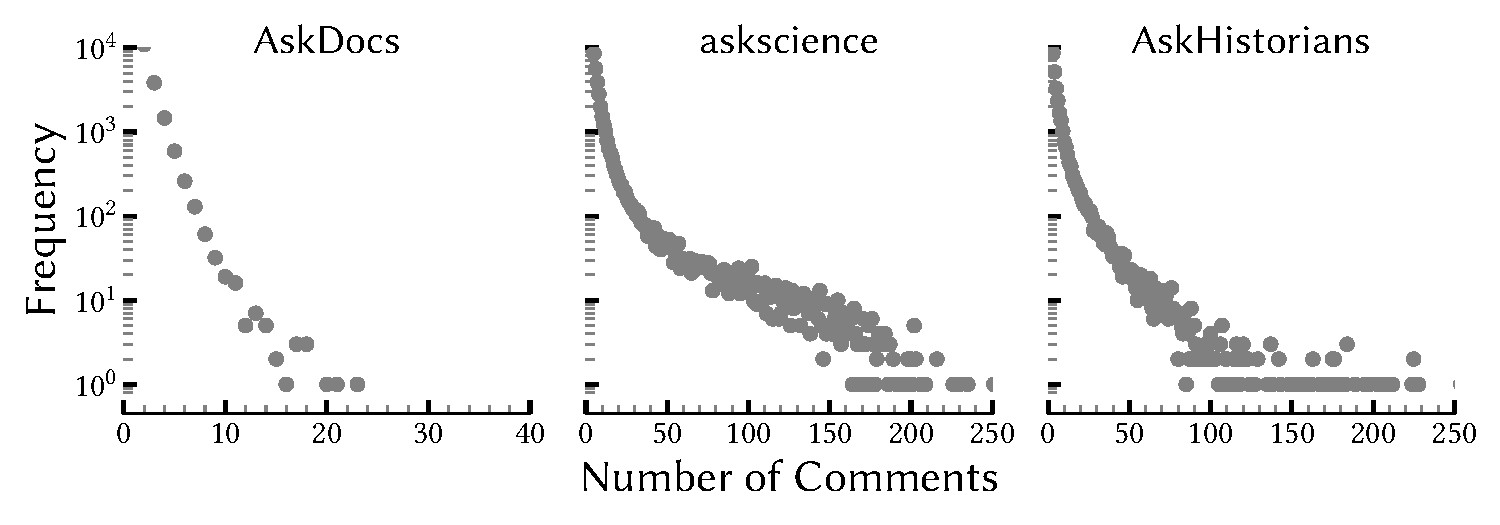
\includegraphics[scale=0.62]{images/Frequency}
  \caption{Frequency plot (log scale) of number of comments per post for three subreddits. A post on AskDocs tend to have fewer comments than the other two communities.}
  \label{fig:frequency}
\end{figure}

For each submission post,
there is a flair text denoting the subtopic of the post, referred as the \textit{submission flair} that is either Moderator added or self-annotated. We denote \emph{submission flair} as the \emph{category} of the post, e.g. Physics, Chemistry, Biology are some categories in AskScience. Similarly, users have \textit{author flairs} attributed next to their user-name, e.g. Astrophysist, Bioengineering. They describe the user's educational background and help the OP in assessing user reliability. In order to get verified and obtain a flair, the users must send the moderators anonymized verification documents, including certification numbers, contact information. We denote verified users with \textit{author flairs} as experts in the rest of the paper.
Table \ref{tab:redditFlairText} presents frequent submission and author flairs for all the subreddits.
AskDocs does not have submission flairs as it is a smaller community.
Figure \ref{fig:flair} shows the distribution of the authors with the number of unique categories of the posts where the user commented. For both subreddits, we observed that around 80\% of the users comment on posts from more than two categories. This shows that users engage with a variety of topics in Reddit.


\begin{table*}[t]
  \centering
\begin{tabular}{ l | p{6cm} | p{6cm}}
\toprule
  Sub-Reddit & Author Flairs & Submission Flairs\\
  \midrule
 *Docs & Physician, Medical Student, Registered Nurse, Physician Assistant, Pharmacist, Nursing Student, Pharmacy Student, EMT, Doctor, Moderator, M.D., Nurse Practitioner     & NA  \\
\hline
 *Science & Biochemistry, Molecular Biology, Immunology, Genetics, Microbiology, Neuroscience, Bioinformatics, Astrophysics, Biophysics, Cell Biology, Materials Science, Cosmology & Physics, Biology, Astronomy, Chemistry, Engineering, Medicine, Earth Sciences, Mathematics, Neuroscience, Computing, Human Body, Planetary Sci. \\
\hline
*Historians & Early Christianity, Ancient Near East, Andean Archaeology, Interesting Inquirer, Colonialism, Mesoamerican Archaeology, New Spain, American Civil War, Holocaust, Medieval Europe, Early Modern Europe, Environment & AMA, Urbanism, Fashion, Myth, Floating, Africa, Literature, Best Of, Pop Music, Home, Death, South America, Trade \\
 \bottomrule
\end{tabular}
%}
\caption{ Top-K most frequent author and submission flairs that appear in our dataset, these flairs are used only in evaluation as our model is unsupervised.  }
\label{tab:redditFlairText}
\end{table*}

Experts are highly active in the community, they answer around 60-70\% of the posts (Table \ref{tab:redditdata}). askscience and AskHistorians have significantly higher and more detailed comments ($\vert w_{m, n} \vert$ in Table \ref{tab:redditdata}) per post than AskDocs, as shown in Figure \ref{fig:frequency}. Due to the prevalence of a large number of comments, manual curation is very expensive, thus necessitating the need for an automatic tool to infer trustworthiness of the comments.

\subsection{Experimental Setup}
We evaluate latent trustworthy comment learned by our model on a trustworthy comment ranking task. That is, given a submission post, our goal is to rank the posted comment based on their trustworthiness.
For this experiment, we treat expert users' comment as the most trustworthy comment of the post.\footnote{While human judgment would be the most precise; it is also the most challenging to collect. For instance, in askscience we would need experts in over 35 science fields, reading up to 250 comments for a single post.}
Besides, we also report results using the highest upvoted comment as the gold standard. Highest upvoted comments represent community consensus on the most trustworthy response for the post \cite{Voting:2019}. While it is shown that there is widespread under-provision on Reddit, and thus, it is possible to miss high-quality content that is not highly voted; nevertheless, upvotes is a good proxy for community consensus~\cite{gilbert2013widespread}.

In particular, we rank comments for each post $m$, in the order of descending cosine similarity between their embedding, $\bm{a}_{m,n}$, and the latent trustworthy comment embeddings, $\bm{a}_m^*$. We then report average Precison@k values over all the posts, where k denotes the position in the output ranked list of comments.


\noindent
\textbf{Baselines:} We compare our model with state-of-the-art truth discovery methods proposed for continuous and text data and non-aspect version of our model. Note that there is no label information used, so we cannot compare to other supervised CQA models \cite{Quality2008,wen2018hybrid,nakov2017semeval} which need this supervision. Our \emph{unsupervised model} is complementary to these approaches, and thus, a rigorous comparison is impossible.


\noindent
\emph{Mean Bag of Answers (MBoA)}: In this baseline, we represent the trustworthy comment for a post as the mean comment embedding. This baseline assumes uniform user reliability.

\noindent
\emph{CRH}: is a state-of-the-art truth discovery-based model for heterogeneous data, i.e. categorical and numerical data~\cite{li2014resolving}. CRH minimizes the weighted deviation of the trustworthy comment embedding from the individual comment embeddings with user reliabilities providing the weights.

\noindent
\emph{CATD}: is an extension of CRH that learns a confidence interval over user reliabilities to handle data skewness~\cite{li2014confidence}. For both the above models, we represent each comment as the average word embeddings of its constituent terms.

\noindent
\emph{TrustAnswer}: Li et al.~\cite{li2017reliable} modeled semantic similarity between comments by representing each comment with embeddings of its key phrase.

\noindent
\emph{CrowdQM-no-aspect:} In this baseline, we condense the commenter's aspect reliabilities to a single $r_n$ and simplify the \emph{user-post reliability} score computation. The updated optimization equation  is,

\begin{equation}
\begin{aligned}
\underset{\{a_m^{*}\}, \{v_{\omega}\}, \{r_n\}  }{\text{min}}
\sum_{n=1}^{N} r_n \left( \sum_{m \in \mathcal{M}_n} s(\bm{u}_{n}, \bm{p}_{m}) \left( E_{m, n} + \beta \odot Q_{m, n} \right) \right)  \\
\text{s.t.  } \sum_{n=1}^{N} e^{-r_n} = 1
\end{aligned}
\end{equation}

This model acts as a control to gauge the performance of our proposed model.

We do not compare with other truth discovery methods ~\cite{Zhao:2012, Yin:2007, Pasternack:2011, Galland:2010, Dong:2009} as CRH and CATD are already shown to outperform them.

\subsection{Results}\label{Results}
Table \ref{tab:pred} reports the Precision@1 results using expert's comments as gold standard.
MBoA, with uniform source reliability, outperforms the CRH method that estimates reliability for each user separately. Thus, simple mean embeddings provide a robust representation for the trustworthy comment.
\begin{table}[tbh]
  \centering
\begin{tabular}{ l | c c c }
\toprule %\hline
 Model &  *Docs & *Science & *Historians \\
  \midrule
 MBoA             & 0.592 & 0.633 & 0.602 \\
 CRH                                     & 0.585 & 0.597 & 0.556 \\
 CATD                                 & \textbf{0.635} & 0.700 & 0.669 \\
 TrustAnswer                     & 0.501 & 0.657 & 0.637 \\
 CrowdQM-no-aspect                           & 0.509 & 0.666 & 0.640 \\
 CrowdQM            & 0.617 & \textbf{0.734} & \textbf{0.753} \\
 \bottomrule
\end{tabular}
% }%
\caption{\label{tab:pred} Precision@1 for all three Ask* subreddits, where the experts' comments are treated as the trustworthy comment. }
\end{table}

We also observe that CrowdQM-no-aspect performs consistently better than TrustAnswer. Note that both approaches do not model aspect-level user reliability but use semantic representations of comments. However, while TrustAnswer assigns a single reliability score for each comment, CrowdQM-no-aspect additionally takes into account the user's familiarity with the post's context (\emph{similarity} function, $s(.)$)
to compute her reliability for the post.
Finally, CrowdQM consistently outperforms both the models, indicating that aspect modeling is beneficial.

CATD uses a confidence-aware approach to handle data skewness and performs the best among the baselines. This skewness is especially helpful in Reddit as experts are the most active users (Table \ref{tab:redditdata}); and, CATD likely assigns them high reliability.
Our model achieves competitive precision as CATD for AskDocs while outperforming for the others. This indicates that our data-driven model works better for communities which are less sparse (Section \ref{subsec:dataset} and Figure \ref{fig:frequency}).

\begin{figure*}[tbh]
\begin{subfigure}{\linewidth}
\centering
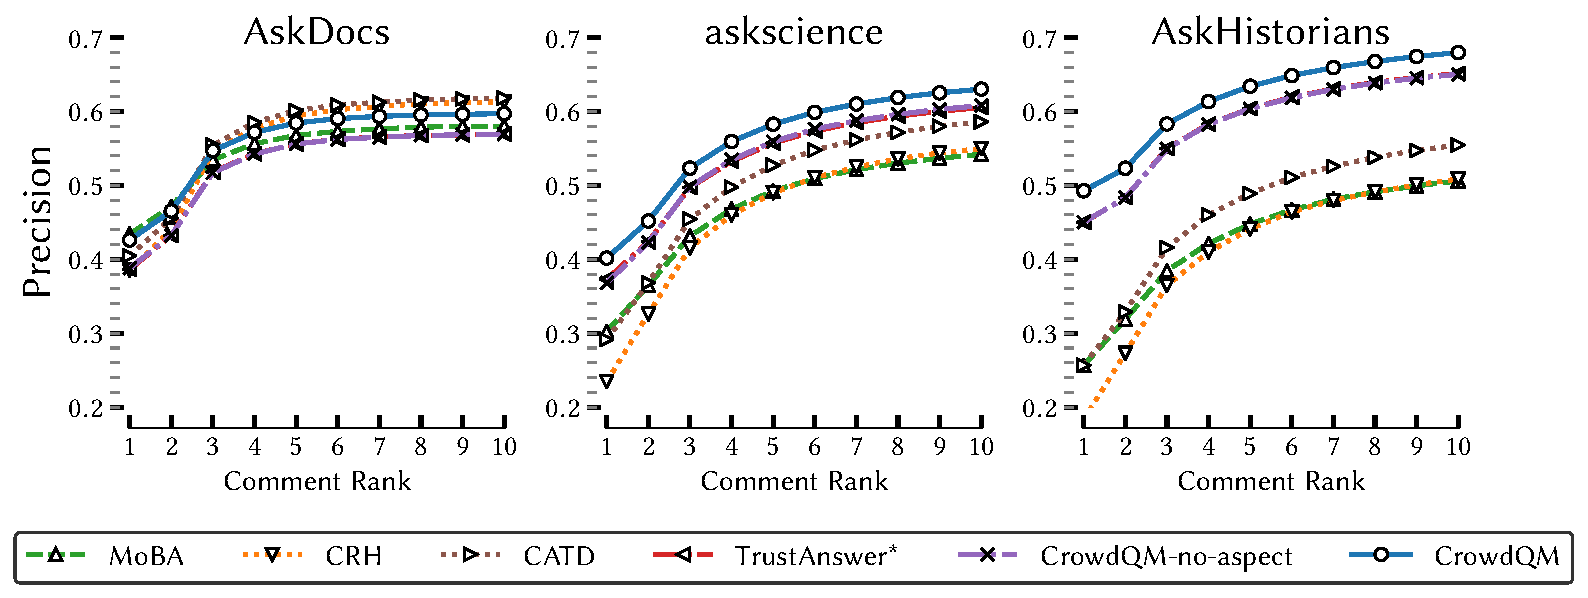
\includegraphics[scale=0.61]{images/Precision.pdf}
\end{subfigure}%
\caption{\label{fig:comment}Precision of our model vs. comment rank computed by user's upvotes. Our model outperforms the baselines for askscience and AskHistorians while performs similarly for AskDocs.}
\end{figure*}

\begin{table}[tbh]
  \centering
\begin{tabular}{l | c c c }
\toprule %\hline
 Model &  *Docs & *Science & *Historians \\
  \midrule
 MBoA                 & \textbf{0.434} & 0.302 & 0.257 \\
 CRH                                         & 0.386 & 0.234 & 0.183 \\
 CATD                                     & 0.405 & 0.291 & 0.257 \\
 TrustAnswer                         & 0.386 & 0.373 & 0.449  \\
 CrowdQM-no-aspect                               & 0.388 & 0.368 & 0.450  \\
 CrowdQM                  & 0.426 & \textbf{0.402} & \textbf{0.493}  \\
 \bottomrule
\end{tabular}
% }%
\caption{\label{tab:pup} Precision@1 for all three Ask* subreddits, where the highest upvoted comment is  treated as the most trustworthy comment.}
\end{table}

Table \ref{tab:pup} reports Precision@1 results using community upvoted comments as the gold standard, while Figure \ref{fig:comment} plots the precision values against the size of the output ranked comment list. In general, there is a drop in performance for all models on this metric because it is harder to predict upvotes as they are inherently noisy~\cite{gilbert2013widespread}.

TrustAnswer and CrowdQM-no-aspect perform best among the baselines indicating that modeling semantic representation is essential for forums. CrowdQM again consistently outperforms the non-aspect based models verifying that aspect modeling is needed to identify trustworthy comments in forums.

CrowdQM remains competitive in the smaller AskDocs dataset, where the best performing model is MoBA. Thus, for AskDocs, the comment summarizing all other comments tends to get the highest votes.

\begin{figure*}[tbh]
\begin{subfigure}{\linewidth}
\centering
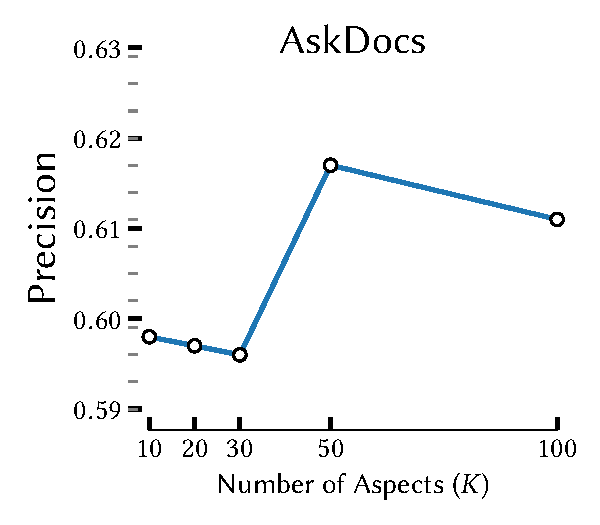
\includegraphics[scale=0.67]{images/Precision_aspect.pdf}
\end{subfigure}
\caption{\label{fig:aspect} Precision of our model with changing number of aspects. Value of $K$ does not have much impact on the precision value.}
\end{figure*}

\textbf{Parameter Sensitivity} In Figure \ref{fig:aspect}, we plot our model's precision with varying number of aspects. Although there is an optimal range around 50 aspects, the precision remains relatively stable
indicating that our model is not sensitive to number of aspects. We also observed similar results for the other datasets and omitted those figures for lack of space. We also did similar analysis with $\beta$ and did not find any significant changes to the Precision.


\subsection{Model Convergence}
\begin{figure}[!h]
\begin{subfigure}{.5\linewidth}
  \centering
  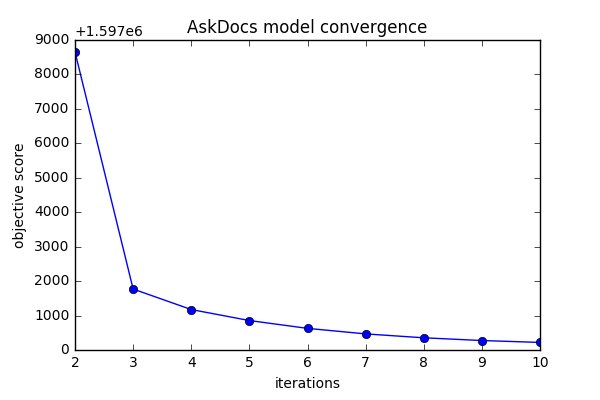
\includegraphics[width=0.9\linewidth]{images/AskDocs_model_convergence.png}
  \caption{AskDocs}
  \label{fig:AskDocsfig1}
\end{subfigure}%
\begin{subfigure}{.5\linewidth}
  \centering
  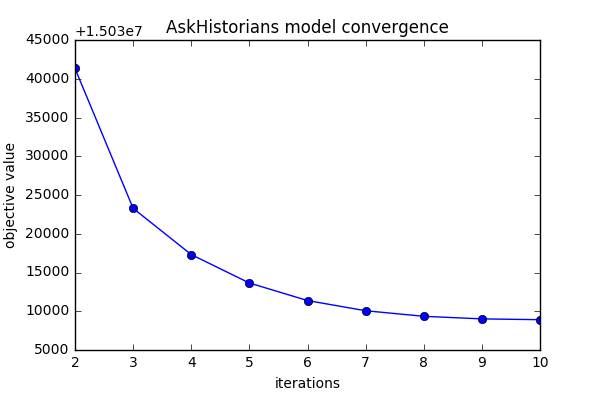
\includegraphics[width=0.9\linewidth]{images/AskHistorians_model_convergence.png}
  \caption{AskHistorians}
  \label{fig:AskHistoriansfig1}
\end{subfigure}
\hspace{6em}
\begin{subfigure}{\textwidth}
  \centering
%   \begin{center}
  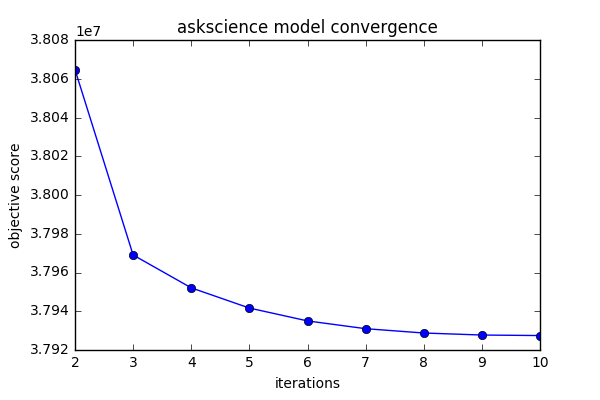
\includegraphics[width=0.49\linewidth]{images/askscience_model_convergence.png}
%   \end{center}
  \caption{askscience}
  \label{fig:asksciencefig1}
\end{subfigure}
\caption{CrowdQM model convergence for AskDocs, AskHistorians, and askscience respectively.}
\label{fig:convergence}
\end{figure}
In Figure \ref{fig:convergence}, we plot the objective function score at each iteration, for our model CrowdQM for the three subreddits. On all three subreddits, the model converges after only about six iterations indicating our model is quick to approximate a solution. In general, the computational complexity is $O(\vert \mathcal{V} \vert N M)$ for a single iteration. However, our implementation leverages the data sparsity in the comment-word usage and user-submissions posts to make the model efficient.
